\section{Homotopy}

  \begin{definition}
    Let $X, Y$ be topological space and let $F_0, F_1: X \longrightarrow Y$ be continuous maps. A \textit{homotopy} from $F_0$ to $F_1$ is a continuous map (with respect to elements $t \in [0,1]$)

      \[H: X \times I \longrightarrow Y\]

    where $I = [0,1]$, satisfying

    \begin{align*}
      & H(x, 0) = F_0 (x) \\
      & H(x, 1) = F_1 (x) 
    \end{align*}

    for all $x \in X$. We can visualize this homotopy as a continuous deformation of (the images of) $F_0$ to $F_1$. We can also think of the parameter $t$ as a "slider control" that allows us to smoothly transition from $F_0$ to $F_1$ as the slider moves from $0$ to $1$, and vice versa. The figures below represents the homotopies between the one-dimensional curves (left) and 2-dimensional surfaces (right), $\im{F_0}$ and $\im{F_1}$, with dashed lines. 

    \begin{center}
    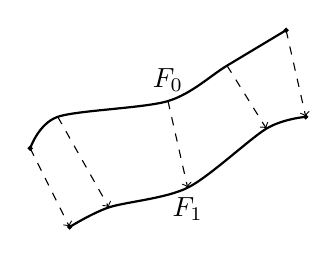
\begin{tikzpicture}[scale=0.5]
      \draw[thick] plot [smooth] coordinates{(-4,0) (-3.3,0.8) (-0.5,1.2) (1,2.1) (2.5,3)};
      \draw[thick] plot [smooth] coordinates{(-3,-2) (-2,-1.5) (0,-1) (2,0.5) (3,0.8)};
      \draw[dashed, ->] (-4,0)--(-3,-2); 
      \draw[dashed, ->] (-3.3,0.8)--(-2,-1.5);
      \draw[dashed, ->] (-0.5,1.2)--(0,-1);
      \draw[dashed, ->] (1,2.1)--(2,0.5);
      \draw[dashed, ->] (2.5,3)--(3,0.8);
      \draw[fill] (-4,0) circle (0.05); 
      \draw[fill] (-3,-2) circle (0.05);
      \draw[fill] (2.5,3) circle (0.05);
      \draw[fill] (3,0.8) circle (0.05); 
      \node[above] at (-0.5,1.2) {$F_0$};
      \node[below] at (0,-1) {$F_1$};
    \end{tikzpicture}
    \end{center}

    If there exists a homotopy from $F_0$ to $F_1$, then we say that $F_0$ and $F_1$ are \textit{homotopic}, denoted

    \[F_0 \simeq F_1\]
  \end{definition}

  \begin{definition}
    If the homotopy satisfies 

      \[H(x,t) = F_0 (x) = F_1 (x)\]

    for all $t \in I$ and $x \in S$, which is a subset of $X$, then the maps $F_0$ and $F_1$ are said to be \textit{homotopic relative to $S$}. 
  \end{definition}

  This is clearly an equivalence relation defined on $C^0 (X, Y)$, the set of all continuous functions from $X$ to $Y$.
  \begin{enumerate}
    \item Identity. Clearly, $F$ is homotopic to itself by setting $H(x, t) \equiv F(x)$ for all $t \in [0,1]$. 

    \item Symmetry. Given homotopy $H(x, t)$ from $F_0$ to $F_1$, the homotopy $H^{-1} (x, t) \equiv H(x, 1-t)$ maps from $F_1$ to $F_0$. 

    \item Transitivity. Given homotopy $H_1$ from $F_1$ to $F_2$, and homotopy $H_2$ from $F_2$ to $F_3$, the homotopy defined

    \[H_3 (x, t) \equiv \begin{cases}
          H_1 (x, 2t) & 0 \leq t \leq \frac{1}{2} \\
          H_2 (x, 2t - 1) & \frac{1}{2} \leq t \leq 1
    \end{cases}\]

    is indeed a homotopy from $F_1$ to $F_3$. 
  \end{enumerate}

  \begin{definition}
  The space of homotopy classes from topological space $X$ to $Y$ is denoted
  \[[X, Y] \equiv \frac{C^0 (X, Y)}{\sim}\]
  where $\sim$ is the homotopy relation. 
  \end{definition}

  \begin{lemma}
  Homotopy is compatible with function composition in the following sense. If $f_1, g_1: X \longrightarrow Y$ are homotopic, and $f_2, g_2: Y \longrightarrow Z$ are homotopic, then $f_2 \circ f_1$ and $g_2 \circ g_1$ are homotopic. That is, given the two homotopies
  \begin{align*}
      & H_1: X \times [0,1] \longrightarrow Y \\
      & H_2: Y \times [0,1] \longrightarrow Z
  \end{align*}
  we can naturally define a third homotopy 
  \[H_3: X \times [0,1] \longrightarrow Z, \; H(x, t) \equiv H_2 (x, t) \circ H_1(x, t)\]
  which is continuous since compositions of continuous functions are continuous. 
  \end{lemma}

  \begin{example}
  If $f, g: \mathbb{R} \longrightarrow \mathbb{R}^2$ is defined as a
  \[f(x) \equiv (x, x^3), \; g(x) \equiv (x, e^x)\]
  then the map 
  \[H: \mathbb{R} \times [0,1] \longrightarrow \mathbb{R}^2, \; H(x, t) \equiv \big( x, (1-t) x^3 + t e^x \big) \]
  is a homotopy between them. 
  \end{example}

  \begin{example}
  Let $id_B: B^n \longrightarrow B^n$ be the identity function on the unit $n$-disk, and let $c_0: B^n \longrightarrow B^n$ be the $0$-function sending every vector to $0$. Then, $id_B$ and $c_0$ are homotopic, with homotopy explicitly defined
  \[H: B^n \times [0,1] \longrightarrow B^n, \; H(x, t) \equiv (1-t) x\]
  \end{example}

  \begin{example}
  If $C \subseteq \mathbb{R}^n$ is a convex set and $f, g: [0,1] \longrightarrow C$ are paths with the same endpoints, then there exists a \textit{linear homotopy} given by 
  \[H: [0,1] \times [0,1] \longrightarrow C, \; (s, t) \mapsto (1-t) f(s) + t g(s)\]
  We can extend this example. Let $f, g: \mathbb{R} \longrightarrow \mathbb{R}$ be 2 continuous functions. Then $f \simeq g$, since we can construct $F: [0,1] \times \mathbb{R} \longrightarrow \mathbb{R}$ defined
  \[F(x, t) \equiv (1-t) f(x) + t g(x)\]
  (Note that the set of continuous functions from $\mathbb{R}$ to $\mathbb{R}$ is a convex set.)
  \end{example}
  This leads to our definition of \textit{path homotopies}, which is just a specific type of homotopy. 

  \begin{definition}
  Suppose $X$ is a topological space. Two paths $f_0, f_1: I \longrightarrow X$ are said to be \textit{path homotopic}, denoted
  \[f_0 \sim f_1\]
  if they are homotopic relative to $\{0, 1\}$. This means that there exists a continuous map $H: I \times I \longrightarrow X$ satisfying
  \begin{align*}
      &H(s, 0) = f_0 (s), \; s \in I \\
      &H(s, 1) = f_1 (s), \; s \in I \\
      &H(0, t) = f_0 (0) = f_1 (0), t \in I \\
      &H(1, t) = f_1 (1) = f_0 (1) , t \in I
  \end{align*}
  \end{definition}
  We can visualize two paths (sharing the same endpoints) being path homotopic if we can "continuously deform" one onto another. 
  \begin{center}
  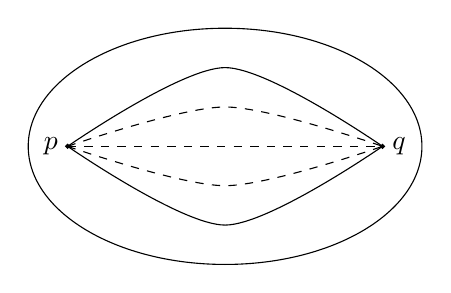
\begin{tikzpicture}[scale=0.5]
      \draw (0,0) ellipse (5 and 3); 
      \draw[fill] (-4,0) circle (0.05); 
      \draw[fill] (4,0) circle (0.05);
      \draw[dashed] (-4,0)--(4,0);
      \draw plot [smooth] coordinates{(-4,0) (0,2) (4,0)};
      \draw[dashed] plot [smooth] coordinates{(-4,0) (0,1) (4,0)};
      \draw[dashed] plot [smooth] coordinates {(-4,0) (0,-1) (4,0)};
      \draw plot [smooth] coordinates {(-4,0) (0,-2) (4,0)};
      \node[left] at (-4,0) {$p$};
      \node[right] at (4,0) {$q$};
  \end{tikzpicture}
  \end{center}
  We can notice that for any given points $p, q \in X$, path homotopy is an equivalence class on the set of all paths from $p$ to $q$. 

  \begin{definition}
  The equivalence class of a path $f$ is called a \textit{path class}, denoted $[f]$. Note that in the diagram above, there is only one equivalence class of paths. 
  \end{definition}

  We can define a multiplicative structure on paths as such. This is the first step to create a group structure on the set of certain paths. 

  \begin{definition}
  Given two paths $f, g$ such that $f(1) = g(0)$, their product is the path defined
  \[(f \cdot g) (s) \equiv \begin{cases}
        f(2s) & 0 \leq s \leq \frac{1}{2} \\
        g(2s - 1) & \frac{1}{2} \leq s \leq 1
  \end{cases}\]
  It is easy to visualize the product of two paths as the longer path created by "connecting" the two smaller paths. 
  \begin{center}
  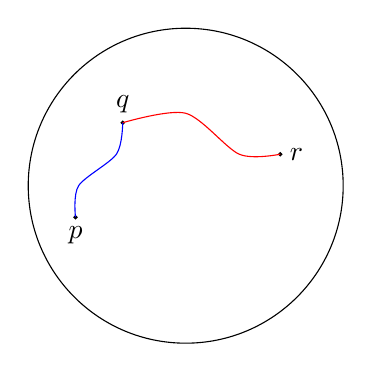
\begin{tikzpicture}[scale=0.4]
      \draw (0,0) circle (5);
      \draw[fill] (-3.5,-1) circle (0.05);
      \draw[fill] (-2,2) circle (0.05);
      \draw[fill] (3,1) circle (0.05);
      \node[above] at (-2,2) {$q$};
      \node[right] at (3,1) {$r$};
      \node[below] at (-3.5, -1) {$p$};
      \draw[blue] plot [smooth] coordinates{(-3.5,-1) (-3.4,0) (-2.2, 1) (-2,2)};
      \draw[red] plot [smooth] coordinates{(-2,2) (0,2.3) (1.7, 1) (3,1)};
  \end{tikzpicture}
  \end{center}
  It is also easy to see that if $f \sim f^\prime$ and $g \sim g^\prime$, 
  \[f \cdot g \sim f^\prime \cdot g^\prime\]
  \end{definition}

  We can also define the product of these equivalence classes as
  \[[f] \cdot [g] \equiv [f \cdot g]\]
  Notice that multiplication of paths is not associative in general, but it is associative up to path homotopy. That is, 
  \[([f] \cdot [g]) \cdot [h] = [f] \cdot ([g] \cdot [h])\]

  \begin{definition}
  If $X$ is a topological space and $q \in X$, a "loop" in $X$ based at $q$ is a path in $X$ such that
  \[f: I\longrightarrow X, \; f(0) = f(1) = q\]
  The set of path classes of loops based at $q$ is denoted
  \[\pi_1 (X, q)\]
  Equipped with the product operation of paths defined before, $(\pi_1 (X, q), \cdot)$ is called the \textit{fundamental group of $X$ based at $q$}. The identity element of this group is the path class of the constant path $c_q(s) \equiv q$, and the inverse of $[f]$ is the path class of 
  \[f^{-1} (s) \equiv f(1-s)\]
  which is the reverse path of $f$. 
  \end{definition}

  Note that while the fundamental group in general depends on the point $q$, it turns out that, up to isomorphism, this choice makes no difference as long as the space is path connected. 

  \begin{lemma}
  Let $X$ be a path connected topological space, with $p, q \in X$. Then, 
  \[\pi_1 (X, p) \simeq \pi_1 (X, q)\]
  for all $p, q$. 
  \end{lemma}

  Therefore, it is conventional to write $\pi_1 (X)$ instead of $\pi_1 (X, q)$ when $X$ is path connected. 

  \begin{example}
  Consider the space $X \equiv B_2 \setminus B_1$, which is the 2-disk without the unit disk in $\mathbb{R}^2$. Given an arbitrary point $p \in X$, there exists an infinite number of path classes of $X$ at $p$, denoted $[p_i]$, where $i$ corresponds to how many times the paths loop around the hole. The first three path classes are shown below. 
  \begin{center}
  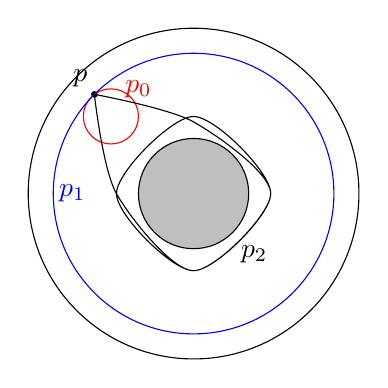
\begin{tikzpicture}[scale=0.7]
      \draw (0,0) circle (3);
      \draw[fill=lightgray] (0,0) circle (1);
      \draw[fill] (-1.8, 1.8) circle (0.05);
      \node[above left] at (-1.75, 1.75) {$p$};
      \draw[red] (-1.5, 1.4) circle (0.5);
      \node[red] at (-1, 1.9) {$p_0$};
      \node[blue] at (-2.2, 0) {$p_1$};
      \node at (1.1, -1.1) {$p_2$};
      \draw[blue] (0,0) circle (2.5455);
      \draw plot [smooth] coordinates{(-1.8, 1.8) (0, 1.3) (1.4, 0) (0, -1.4) (-1.4, 0) (0, 1.4) (1.4, 0) (0, -1.4) (-1.4, 0) (-1.8, 1.8)};
  \end{tikzpicture}
  \end{center}
  It is clear that $[p_0]$ is the identity, and the group operation rule is
  \[[p_i] \cdot [p_j] = [p_{i+j}]\]
  meaning that $\pi_1(X, p)$ is the infinite discrete group generated by $[p_0]$ and $[p_1]$. 
  \end{example}

  \begin{proposition}
  Let $\mathcal{A}$ be a convex subset of $\mathbb{R}^n$, endowed with the subspace topology, and let $X$ be any topological space. Then, any 2 continuous maps $f,g: X \longrightarrow \mathcal{A}$ are homotopic. 
  \end{proposition}
  \begin{proof}
  Since $\mathcal{A}$ is convex, the homotopy defined 
  \[F(x, t) \equiv (1-t) f(x) + t g(x)\]
  exists. 
  \end{proof}

  \begin{proposition}
  If $X$ is a path connected space, the fundamental groups based at different points are all isomorphic. That is, 
  \[\pi_1 (X, p) \simeq \pi_1 (X, q)\]
  for all $p, q \in X$. 
  \end{proposition}

  \begin{definition}
  If $X$ is path connected and for some $q \in X$, the group $\pi_1 (X, q)$ is the trivial group consisting of $[c_q]$ alone, then we say that $X$ is \textit{simply connected}. By definition, this means that every loop is path homotopic to a constant path. 
  \end{definition}

  \begin{proposition}
  Let $X$ be a path connected topological space. $X$ is simply connected if and only if any 2 loops based on the same point are path homotopic. 
  \end{proposition}

  We can also expect that since homotopy is clearly a topological property, it is preserved under continuous maps. We state this result formally in the following lemma.

  \begin{lemma}
  If $F_0, F_1: X \longrightarrow Y$ and $G_0, G_1: Y \longrightarrow Z$ are continuous maps such that $F_0 \simeq F_1$ and $G_0 \simeq G_1$, then 
  \[G_0 \circ F_0 \simeq G_1 \circ F_1\]
  Similarly, if $f_0, f_1: I \longrightarrow X$ are path homotopic, and $F: X \longrightarrow Y$ is a continuous map, then 
  \[F \circ f_0 \sim F \circ f_1\]
  Thus, if $F: X \longrightarrow Y$ is a continuous maps, for each $q \in X$, we can construct a well-defined map
  \[F_*: \pi_1 (X, q) \longrightarrow \pi_1 \big( Y, F(q)\big)\]
  by setting
  \[F_* ([f]) \equiv [F \circ f]\]
  \end{lemma}

  \begin{lemma}
  If $F: X \longrightarrow Y$ is a contiuous map, then the induced map 
  \[F_* : \pi_1(X, q) \longrightarrow \pi_1 \big( Y, F(q)\big)\]
  is a group homomorphism. 
  \begin{tikzpicture}
      \node at (0,0) {x};
  \end{tikzpicture}
  That is, $F_*$ preserves multiplicative structure of the loops. 
  \end{lemma}

  \begin{theorem}[Properties of the Induced Homomorphism]
  \begin{enumerate}
      \item Let $F: X \longrightarrow Y, G: Y \longrightarrow Z$ be continuous maps. Then for any $q \in X$, 
      \[(G \circ F)_* = G_* \circ F_* : \pi_1 (X, q) \longrightarrow \pi_1 \big(Z, G(F(q))\big)\]
      \item For any space $X$ and any $q \in X$, the homomorphism induced by the identity map $id_X: X \longrightarrow X$ is the identity map 
      \[id: \pi_1 (X, q) \longrightarrow \pi_1 (X, q)\]
      \item If $F: X \longrightarrow Y$ is a homeomorphism, then 
      \[F_* : \pi_1 (X, q) \longrightarrow \pi_1\big( Y, F(q)\big)\]
      is an isomorphism. That is, homeomorphic spaces have isomorphic fundamental groups.  
  \end{enumerate}
  \end{theorem}

  \begin{example}
  The fundamental group of $S^1 \subset \mathbb{C}$ based at $0$ is the infinite cyclic group generated by the path class of the loop
  \[\alpha: I \longrightarrow S^1, \; \alpha(s) \equiv e^{2 \pi i s}\]
  \end{example}

  \begin{theorem}
  If $F: X \longrightarrow Y$ is a homotopy equivalence, then for each $p \in X$, 
  \[F_* : \pi_1 (X, p) \longrightarrow \pi_1 \big( Y, F(p) \big)\]
  is an isomorphism. 
  \end{theorem}

  The following proposition will be revisited when studying manifolds. 

  \begin{proposition}
  The fundamental group of any topological manifold is countable. 
  \end{proposition}

\subsection{Homotopy Equivalence}

  \begin{definition}
  Given two topological spaces $X$ and $Y$, a homotopy equivalence between $X$ and $Y$ is a pair of continuous maps $f:X \longrightarrow Y$ and $g: Y \longrightarrow X$ such that 
  \[g \circ f \simeq id_X \text{ and } f \circ g \simeq id_Y\]
  The equivalence classes under $\simeq$ are called \textit{homotopy types}. If such a pair $f, g$ exists, $X$ and $Y$ are said to be \textit{homotopy equivalent}, or of the same homotopy type. 
  \end{definition}

  \begin{definition}
  Spaces that are homotopy equivalent to a point are called \textit{contractible}. That is, $X$ is contractible if and only if 
  \[X \simeq \{x_0\}\]
  \end{definition}

  Visually, two spaces are homotopy equivalent if they can be transformed into one another by bending, shrinking, and expanding operations. 

  \begin{example}
  A solid disk is homotopy equivalent to a single point, since one can deform the disk along radial lines to a point. 
  \end{example}

  \begin{example}
  A mobius strip is homotopy equivalent to a closed (untwisted) strip. 
  \end{example}

  Notice from the visualization of homotopy equivalence the following proposition. 

  \begin{proposition}
  $X, Y$ homeomorphic $\implies$ $X, Y$ homotopy equivalent. However, the converse is not true. 
  \end{proposition}
  \begin{proof}
  Just set $f = f$ and $g = f^{-1}$. 
  \end{proof}

  \begin{example}
  A torus is not homotopy equivalent to $Y$, which also implies that they are not homeomorphic either. 
  \begin{center}
  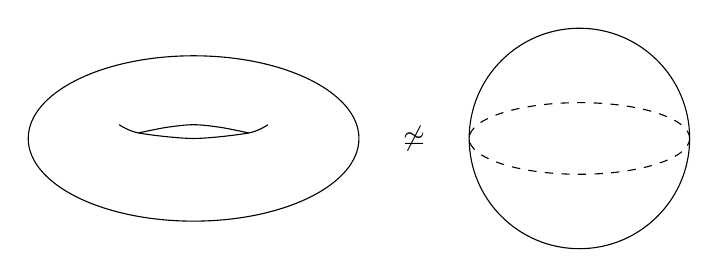
\begin{tikzpicture}[scale=0.35]
      \draw (0,0) ellipse (6 and 3);
      \draw plot [smooth] coordinates{(2.7,0.5) (2, 0.2) (0,0) (-2, 0.2) (-2.7, 0.5)};
      \draw plot [smooth] coordinates{(2, 0.2) (1, 0.4) (0, 0.5) (-1, 0.4) (-2, 0.2)};
      \draw (14,0) circle (4);
      \draw[dashed] (14,0) ellipse (4 and 1.3);
      \node at (8,0) {$\not\simeq$};
  \end{tikzpicture}
  \end{center}
  \end{example}

  Furthermore, like homeomorphisms, homotopy equivalence is a relation on the set of all topological spaces. 
  \begin{enumerate}
      \item Identity. Just set $f, g = id_X$
      \item Symmetricity. Given $X \simeq Y$ with $f: X \longrightarrow Y, g: Y \longrightarrow X$, we set $f^\prime \equiv g$ and $g^\prime \equiv f$ and use these functions $f^\prime, g^\prime$ to find out that $Y \simeq X$. 
      \item Transitivity. Let us have $X \simeq Y$ with functions $f_1, g_1$ and $Y \simeq Z$ with functions $f_2, g_2$. Then, we define new functions 
      \[f_3 \equiv f_2 \circ f_1: X \longrightarrow Z, \; g_3 \equiv g_1 \circ g_2: Z \longrightarrow X\]
      which follows to $f_3 \circ g_3 = id_Z$ and $g_3 \circ f_3 = id_X$. 
  \end{enumerate}

  \begin{proposition}
  $\mathbb{R}^n$ is homotopically equivalent to a point $\{0\}$.
  \end{proposition}
  \begin{proof}
  We claim that the continuous maps (canonical injection and projection)
  \[id_{\mathbb{R}^n}: \{0\} \longrightarrow \mathbb{R}^n , \; p_0 : \mathbb{R}^n \longrightarrow \{0\}\]
  have the property that 
  \[id_{\mathbb{R}^n} \circ p_0 \simeq id_{\mathbb{R}^n} , \; p_0 \circ id_{\mathbb{R}^n} \simeq id_{\{0\}}\]
  The right-hand homotopy is trivial since $id_{\mathbb{R}^n} \circ p_0 = id_{\mathbb{R}^n}$, and as for the left-hand homotopy, we can explicitly define it as
  \[H: [0,1] \times \mathbb{R}^n \longrightarrow \mathbb{R}^n\]
  with
  \[H(t, x) \equiv (t) (id_{\mathbb{R}^n} \circ p_0 )(x) + (1-t) \, id_{\mathbb{R}^n} (x) = (1-t)\, id_{\mathbb{R}^n} (x)\]
  \end{proof}

  \begin{example}
  $S^1 \simeq \mathbb{R}^2 \setminus \{0\}$, and more generally, $S^{n-1} \simeq \mathbb{R}^n \setminus \{0\}$. We can see this with the canonical injection and projections
  \[id_{\mathbb{R}^2}: S^1 \longrightarrow \mathbb{R}^2 \setminus \{0\}, \; \pi_{S^1}: \mathbb{R}^2 \setminus \{0\} \longrightarrow S^1\]
  and find that
  \[id_{\mathbb{R}^2} \circ \pi_{S^1} \simeq id_{\mathbb{R}^2}, \; \pi_{S^1} \circ id_{\mathbb{R}^2} \simeq id_{S^1}\]
  where the right-hand homotopy is trivial, and the left hand homotopy is defined explicitly as
  \[H(x, t) \equiv t (id_{\mathbb{R}^2} \circ \pi_{S^1})(x) + (1-t) (id_{\mathbb{R}^2})(x)\]
  \end{example}

  \begin{definition}
  A function $f$ is said to be \textit{null homotopic} if it is homotopic to a constant function. This is sometimes called a \textit{null-homotopy}. 
  \end{definition}

  \begin{example}
  Take a look at a function $f: \mathbb{R}^2 \longrightarrow \mathbb{R}$, which represents an arbitrary surface in $\mathbb{R}^2 \oplus \mathbb{R}$. Now, observe the constant function $c(x, y) \equiv c$, which represents a plane parallel to the $x, y$-plane. Clearly, we can imagine a deformation of the surface of $f$ to the flat surface of $c$ with the homotopy
  \[H(x, t) \equiv t \, f(x) + (1-t) c(t)\]
  which visually represents a linear deformation of $c$ to $f$. Therefore, $f$ is null-homotopic. 
  \end{example}

  \begin{example}
  A map $f: S^1 \longrightarrow X$ is null homotopic precisely when it can be continuously extended to a map 
  \[\Tilde{f}: D^2 \longrightarrow X\]
  that agrees with $f$ on the boundary $\partial D^2 = S^1$. Visually, the existence of $\Tilde{f}$ allows us to continuously deform the image of $f$ in $S^1 \oplus X$ to a level curve $f(x) = c$ existing in $S^1 \oplus X$. 
  \end{example}

  \begin{proposition}
  A space $X$ is contractible if any only if the identity map from $X$ to itself, which is always a homotopy equivalence, is null homotopic. 
  \end{proposition}

  \begin{example}
    Let $Y$ be the following gray subset of the plane, and let $X$ be the figure-8 shape. 
    \begin{center}
    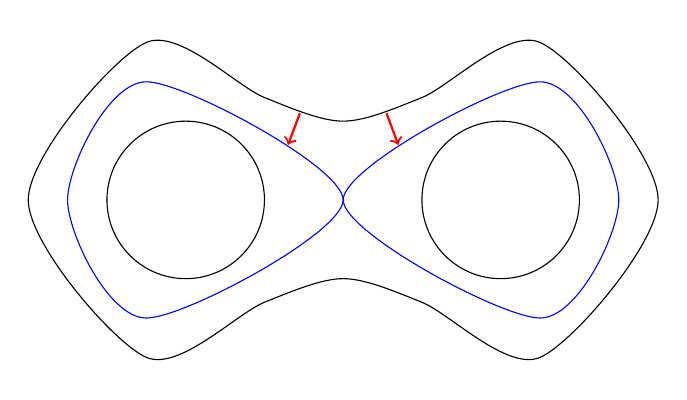
\begin{tikzpicture}
      \draw (-2,0) circle (1);
      \draw (2,0) circle (1);
      \draw[blue] plot [smooth cycle] coordinates{(0,0) (-2.5, 1.5) (-3.5, 0) (-2.5, -1.5)};
      \draw[blue] plot [smooth cycle] coordinates{(0,0) (2.5, 1.5) (3.5, 0) (2.5, -1.5)};
      \draw plot [smooth cycle] coordinates{(0, 1) (1,1.3) (2.5, 2) (4,0) (2.5, -2) (1, -1.3) (0, -1) (-1, -1.3) (-2.5, -2) (-4, 0) (-2.5, 2) (-1, 1.3)};
      \draw[thick, red, ->] (0.55, 1.1)--(0.7,0.7);
      \draw[thick, red, ->] (-0.55, 1.1)--(-0.7,0.7);
    \end{tikzpicture}
  \end{center}
  Then $Y \simeq X$, where the corresponding functions are
  \begin{align*}
      & F: X \longrightarrow Y, \text{ the canonical inclusion} \\
      & F: Y \longrightarrow X, \text{ the projection onto X}
  \end{align*}
  Then, $G \circ F = id$ and $F \circ G$ is homotopic to the identity, with homotopy defined
  \[H(x, t) \equiv t (F \circ G) (x) + (1-t) (id_Y) (x)\]
  which can be visualized by $H(x, s)$ being the point you get from $x$ by moving a fraction $s$ along the red arrow towards $X$. 
  \end{example}

